%
% File: chap03.tex
% Author: Oliver J. H. Feighan
% Description: Theory and parameterization for chl-xTB method. 
% Include vibronic PES tests, and absorption spectra.
%
\let\textcircled=\pgftextcircled
\chapter{Chlorophyll specific methods}
\label{chap:chl_xtb}

\initial {T}his chapter reports the work done on designing and parameterising a
novel method for response properties. The framework and theory for the method is
outlined in section \ref{sec:theory}. Parameterisation details are given in 
section \ref{sec:chl_params}, including the reference data that compromised the 
training data, the objective function used and the algorithms that were used for
optimisation. The accuracy of this new method is showcased in the final section 
\ref{sec:chl_benchmarking}.

%=======
\section{Theory}
\label{sec:theory}
Excitations from linear-response TD-DFT are given by solving the non-Hermitian
eigenvalue equation:

\begin{equation}
    \begin{pmatrix}
        \mathbf{A}   & \mathbf{B} \\
        \mathbf{B}^\ast  & \mathbf{A}^\ast
    \end{pmatrix}
    \begin{pmatrix}
        \mathbf{X} \\
        \mathbf{Y}
    \end{pmatrix}
    = 
    \omega
    \begin{pmatrix}
        1 & 0 \\
        0 & -1
    \end{pmatrix}
    \begin{pmatrix}
        \mathbf{X} \\
        \mathbf{Y}
    \end{pmatrix}
\end{equation}

where $\mathbf{A}$, $\mathbf{B}$ are matrices whose elements describe the perturbation
response of the electron density. $\mathbf{X}$, $\mathbf{Y}$ solutions are the 
coefficients of excitations, similar to CIS, and eigenvalues $\omega$ are the 
excitation energies.

The elements of $\mathbf{A}$ and $\mathbf{B}$ correspond to descriptions of the
virtual-occupied and occupied-virtual elements respectively, and in TD-DFT, with a 
global hybrid density functional, are given by:

\begin{equation}
A_{ia,jb} = \delta_{ij} \delta_{ab} \left( \epsilon_a - \epsilon_i \right) + 2\left(ia|jb\right) - a_x\left(ij|ab\right) + (1- a_x)\left(ia|f_{\text{XC}}|jb\right)
\end{equation}

\begin{equation}
B_{ia,jb} = 2\left(ia|bj\right) - a_x\left(ib|aj\right) + (1- a_x)\left(ia|f_{\text{XC}}|bj\right)
\end{equation}

where indices $a,b$ and $i,j$ refer to virtual and occupied orbitals respectively, 
$a_x$ is the value of non-local Fock exchange in the XC functional $f_{\text{XC}}$.
The intergral (here in Mulliken notation) can be seen to be of Coloumb type for 
the $\mathbf{A}$ matrix and exchange for the $\mathbf{B}$ matrix.

\subsection{Approximations to Solutions}
\label{subsec:chl_approxs}

\subsubsection{Tamm-Dancoff Approximation and Diagonal Dominant $\mathbf{A}$ matrices}
\label{subsubsec:Tamm_Dancoff}

One of the earliest approximations applied to full TD-DFT was the Tamm-Dancoff
approximation, where only virtual-occupied effects were taken into account. This
sets all of the elements of $\mathbf{B}$ matrix to zero, and reduces the full
eigenvalue equation to 

\begin{equation}
\mathbf{A} \mathbf{X} = \omega \mathbf{X}
\end{equation}

where the definitions of elements are the same as above, but it should be noted 
that the solutions $\mathbf{X}$ will be not be same. This is formally the same as
a CIS problem, and has been reported as a way to get back to CIS from full
TD-DFT.

As an eigenvalue problem, the way to solve for $\omega$ is to construct the full
$\mathbf{A}$ and then diagonlise. Additionally, this is required as the XC functional
is dependent on $\omega$ values and so several iterations of this diagonalisation 
are needed to find stable, self-consistent solutions.

However, the diagonal elements of the $\mathbf{A}$ matrix may be an approximation
to the eigenvalue solutions. This would be in the limit where the coupling elements,
the off-diagonal elements, go to zero, which would be the case for an excitation that
is mostly made up of a single transition. Excitation energies therefore would
be given by:

\begin{equation}
\omega_{ia} = A_{ia, ia} = \left( \epsilon_a - \epsilon_i \right) + 2\left(ia|ia\right) - a_x\left(ii|aa\right) + (1- a_x)\left(ia|f_{\text{XC}}|ia\right) 
\label{eq:diag_dom}
\end{equation}

. If the integrals are assumed to also be small compared to the first term difference 
of $\epsilon_a$ and $\epsilon_i$, then the excitation energy would then be equal
to just this eigenvalue difference, hence its use as a proxy for higher-level
TD-DFT.

\subsection{Integrals approximations}
\label{subsec:MNOK}

The two electron integrals as written above are usually one of the most expensive
part of a calculation. These can be approximated with a monopole expansion, treating
atomic sites as charges, and using a charge-charge interaction for the energy.
A L{\"o}wdin population scheme can be used to obtain the atomic (centered on atom
$A$) charges densities $q^A_{nn}$ and transition charge densities $q^A_{nm}$:

\begin{equation}
q^A_{nm} = \sum_{\mu \in A} C^\prime_{\mu n} C^\prime_{\mu m}
\end{equation}

where $\mu$ are indices of AOs centered on atom $A$, and $\mathbf{C}^\prime$ are the 
orthogonalised MO coefficients, following the same orthogonalisation scheme as 
previously used:

\begin{equation}
\mathbf{C}^\prime_n = \mathbf{S}^{\frac{1}{2}} \mathbf{C}_n
\end{equation}

where $\mathbf{S}$ are the AO overlaps, and $\mathbf{C}$ the unorthogonalised orbitals.

The two electron integrals can be approximated by using MNOK integrals. For both 
coloumb and exchange type integrals, this is done with a short-range damped MNOK
operators. The integral is approximated by:

\begin{equation}
\left(pq|rs\right) = \sum^N_A \sum^N_B q^A_{nm} q^B_{nm} \Gamma_{AB}
\end{equation}

where $N$ is the total number of atoms in the system, $p$,$q$,$r$ and $s$ electron
indices. For Coloumb type integrals, the operator $\Gamma_{AB}$ is given by:

\begin{equation}
\Gamma^J_{AB} = \left(\frac{1}{\left(R_{AB}\right)^{y_J} + \left(a_x \eta\right)^{-y_J}} \right)^{\frac{1}{y_J}}
\end{equation}

where $R_AB$ is the interatomic distance of atoms $A$, $B$, $\eta$ is the average
of the chemical hardness of atoms $A$ and $B$. These values are defined as:

\begin{equation}
\eta\left(A\right) = \frac{\delta^2 E\left(A\right)}{\delta^2 N^2}
\end{equation}

but in practice are precomputed and used as parameters. $y_J$ is a global parameter
and usually set to integer values. $a_x$ is the previously defined amount of Fock-exchange
mixing.

For exchange type, the operator is:

\begin{equation}
\Gamma^K_{AB} = \left(\frac{1}{\left(R_{AB}\right)^{y_K} + \eta^{-y_K}} \right)^{\frac{1}{y_K}}
\end{equation}

where the $y_K$ parameter replaces the $y_J$ parameter in the Coloumb type operator.

As the $a_x$ parameter can "mop up" many of the exchange effects, the density functional
in equation \ref{eq:diag_dom} is also neglected to further reduce computational cost.

The final form of the expression used to calculated excitation energies is then
given by:

\begin{equation}
A_{ia,ia} = \left(\epsilon_a - \epsilon_i\right) + \sum^N_{A,B}\left(2 q_{ia}^A \Gamma^K_{AB} q_{ia}^B - q^A \Gamma^J_{AB} q^B\right)
\end{equation}

where the exchange term uses transition charges $q_{ia}$, and the coloumb term uses
normal charges.

The approximations outlined so far have been based on both the sTDA \cite{Grimme2013}
and sTDA-xTB \cite{Grimme2016} methods, which show great success at both reducing the 
amount of computational cost as well as accurately predicting transition properties
for small molecules and larger systems.

\subsection{\Qy Transition}
\begin{figure}
    \centering
    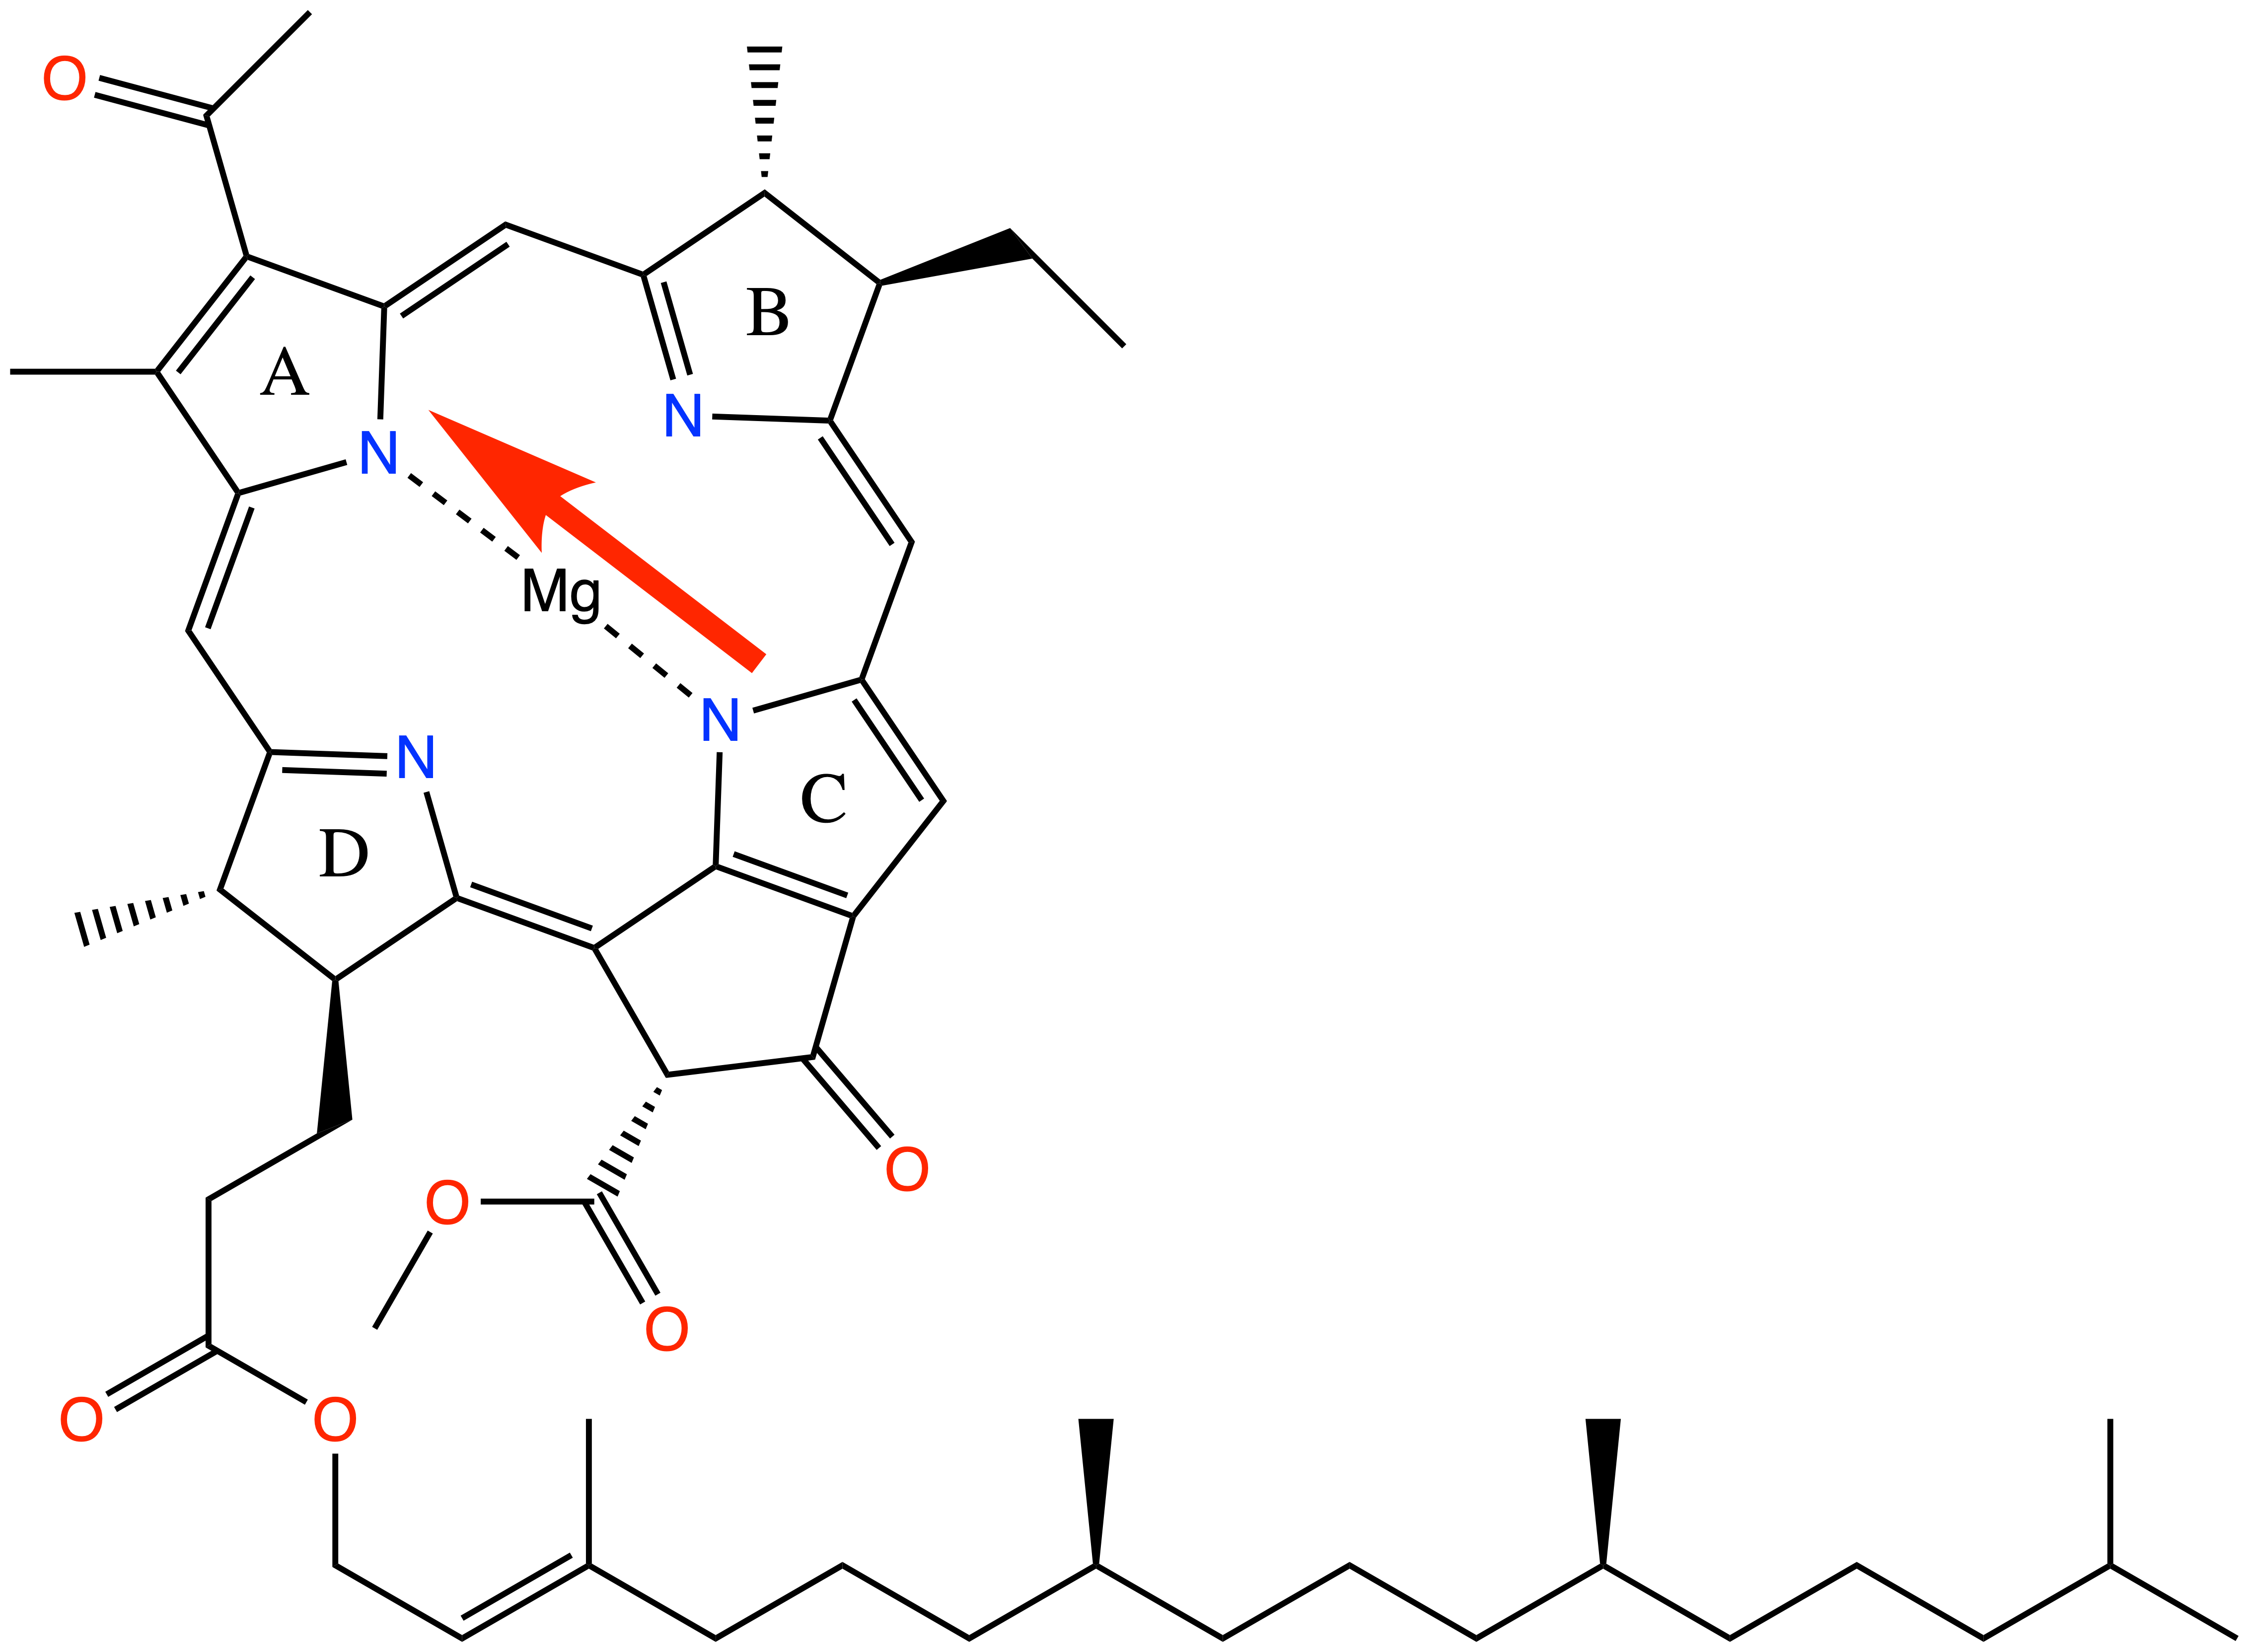
\includegraphics{chapters/chapter03/chlorophyll_Qy.png}
    \caption{Bacterial Chlorophyll a (BChla) with a model \Qy transition dipole.}
    \label{fig:bchla_qy}
\end{figure}

The \Qy transition is the one of the two transitions that make up
the $Q$ band in the absorption spectra of chlorophyll, the other being the $Q_x$
transition. It is well known that the \Qy transition is important for electronic 
energy transfer, as predicting both transition energies and transition dipole 
magnitudes and orientations is important to construct frameworks for this transfer.
The \Qy transition is mostly HOMO-LUMO in character (~96\%), with a small amount of HOMO-1
- LUMO+1 (remaining 4\%). The analogous transition in the unsubstituted tetraphorphyrin
ring has the transition dipole along the molecular axis defined by the N atoms,
however due to the asymmetry introduced by substitutions and geometry deformations,
this is usually not the case for BChla by around 12 $^{\circ}$.

Plots of the electron density of the HOMO, LUMO and transition density show how
this transition is delocalised over large sections of the porphyrin ring, with 
approximate $C_2$ symmetry along the molecular axes.

It has recently also been shown that the high correlation between the eigenvalue
difference of HOMO-LUMO orbitals and full TD-DFT excitation energies implies that
the HOMO-1 - LUMO+1 transition can be excluded from the transition character. This
is also supported by the chlorophyll data in the previous chapter.

\subsection{chl-xTB method}
\label{subsec:chl_method}
This section will set out the novel procedure for calculating transition properties
for chlorophyll, which is named chlorophyll-xTB, abbreviated to chl-xTB.

This method, in the form reported here, is specific to the \Qy transition for 
bacterial chlorophyll A systems. This transition constitutes the entire training
set, and the validity of this method outside of this range is not tested. This is
due to the aim that this method could predict variations in values for transition
properties that would be due to atomic geometry reasons, which is a high level of
specificity.
Initially it was investigated whether this method could be applicable to a broad
range of systems and transitions. However it was found that parameter optimisation
procedures, whilst improving upon the accuracy of the \dxtb methods of the previous
chapter, could not break into the accuracy needed to correctly predict geometry variations.
Additionally, by reducing the scope of systems, the specificity of parameters can
dramatically increase. This reduces the need to include more parameters to improve
accuracy, as well as decreasing the amount of training data needed. It is
argued that this is an improvement on a broader method, that would have been much
harder and more expensive to train.

The first part of the chl-xTB method was to adjust the electronic structure method
for a better starting ground state density. As shown in the previous chapter, this
was an issue with the \dxtb methods. The GFN1-xTB Fock matrix is made of both charge
depenedent and charge independent terms, and only the charge dependent terms would
have any effect on the transition properties as these would effect the partial and
transition charges. The charge dependent terms are the first, second and third 
density fluctuation terms. The first order term is the leading term, and so the 
these parameters were chosen to be included in the optimisation procedure. Of these,
only certain parameters are "free", as in based on the top-down method of parameterisation,
whilst others are based on physical or \emph{ab initio} values. One set of free parameters 
which were altered for this method are the H{\"u}ckel parameters $k_l$, where $l$
is the angular momentum of the orbital, and the global scaling parameters. In the
original GFN1-xTB method there are also free parameters called global scaling 
parameters, which were used to adjust for some pairs of elements were the general
procedure led to incorrect bond lengths. Similar parameters were also included, but
only for the Mg and N atoms. Whilst other atoms types could have been part of this
global scaling scheme, it was found that only these two were necessary to achieve
a decent the accuracy. Using this small amount of parameters would reduce the risk
of overfitting to the training set.
An obvious drawback of altering these parameters to fit to transition properties
is that they would lose their specificity to geometry optimisation and normal-frequencies,
as well as to the non-covalent interactions although should be less effected. However
it is not in the scope of this work to find a semi-empirical method to do be able
to calculate these properties for chlorophyll. The chl-xTB is not used to calculate
optimised geometries or hessians of chlorophyll as other methods could be expected 
to perform better. Also if this were the necessary, including more target properties
in the parameter optimisation would decrease the accuracy to any one target, making
the method worse overall. For example, the sTDA-xTB and GFN-xTB methods use different
electronic structure parameters for this reason.

The second part of this method calculate the transition density based on a \dscf
like approach to the excited state density, but without orbital relaxation. The
ground state orbital coefficients are taken to be a good approximation to the
(\Qy) excited state coefficients. The transition density is then calculated as:

\begin{equation}
D_{Q_y}
\end{equation}

. This is then used to calculate the transition charges with the Mulliken scheme,
which is in turn used to calculate the MNOK integrals of the form eq.
Here the free parameters $a_x$, $y_J$, $y_K$ are optimised specific to the \Qy 
transitions, whilst $\eta$ is calculated using the GFN1-xTB chemical hardnesses for
consistency, as well as to avoid overfitting. Similar to \dscf, the transition dipoles 
can be calculated as the trace of the dipole operator with the transition density:

It should be noted the ground and excited states would be orthogonal in this scheme,
as they share the same set of MO coefficients. Additionally, only one cycle of the
SCC procedure would be necessary, which would eliminate the problem of convergence
in the \dscf excited state. It would also halve the computational time.
Excited state properties, such as the molecular dipole and partial charges can
also be calculated as the excited state density can be constructed in a similar 
fashion, which will be important for the exciton framework of the next chapter.

It's clear that this method is heavily inspired by sTDA-xTB.
However there are some key differences in this theory that constitutes novel work.
The most obvious is the ground state method. sTDA-xTB uses a bespoke version of
the xTB formalism, which whilst similar has some key differences. These include 
the use of a geometry dependent basis set, whereas the chl-xTB method uses a fixed
basis set. The Fock matrix terms for chl-xTB are also different, and for the most
part the same as GFN1-xTB, with the notable exception of the extended H{\"u}ckel
term which uses novel chl-xTB specific parameters. Third is the SCC procedure, which
is is replaced in sTDA-xTB for single diagonlastions.
First is that the sTDA methods still solve the eigenvalue problem, and so require
constructing the entire $\mathbf{A}$ matrix. As stated earlier, it is assumed for
transitions were the corresponding sections of the $\mathbf{A}$ matrix are diagonal
dominant this is unnecessary. Additionally, instead of the L{\"o}wdin scheme for
atomic charges, the Mulliken scheme was used. This gives the charges centered
on atom $A$ as:

\begin{equation}
q^A = Z_A - \sum_{\mu \in A} D_{\mu\nu} S_{\mu\nu}
\end{equation}

where $\mathbf{D}$ is the reduce one-electron density, and $Z_A$ is the atomic number.
For transition charges, this density can be switch with the transition density. 
The choice to use Mulliken charges over L{\"o}wdin charges was made due to the known
instability of L{\"o}wdin charges with respect to orbital rotation, however it is
known that Mulliken charges are highly dependent on the basis set chosen. 

Additionally, a scaling factor for the transition density was employed to attempt
to recover some of the effects of neglecting off diagonal elements from the $\mathbf{A}$
matrix.

\afterpartskip
\section{Parameterization}
\label{sec:chl_params}
\subsection{Reference Data}
\label{subsec:ref_data}
The geometries for the training set used to optimise the chl-xTB method were taken
from previously done classical MD of the LHII protein. These geometries were chosen
as the stochastic variations of the BChla molecules would represent a range of
configurations, which would train chl-xTB to accurately predict variations of 
transition properties on vibrational modes.

Transition properties were calculated with a range of methods, covering levels of
theory that would be comparable to the chl-xTB formalism. These included an eigenvalue
difference approach, \dscf, and three levels of TD-DFT. 

Training the chl-xTB parameters was done against the PBE0 data. This data was chosen
for the best accuracy-cost ratio, as well as having been previously used to investigate
exciton properties for the LHII system. Additionally, from the outset it was unknown
how much training data would be necessary, and so keeping potential future costs
of expanding the training data down was another factor in choosing this functional.

\begin{figure}
    \includegraphics{../../Year_2/chlorophyll_parameterization/tddft_data/ResponseMethodsEnergiesCorrelations.png}
    \caption{correlations of energies}
\end{figure}

\begin{figure}
    \includegraphics{../../Year_2/chlorophyll_parameterization/tddft_data/ResponseMethodsTDMSCorrelations.png}
    \caption{correlations of transition dipole moments}
\end{figure}

\subsection{Objective Function}
\label{subsec:obj_func}
The design of the objective function, the function that is minimised in the optimisation
procedure, is also important to find the best parameters.

At first, it would be argued that the root mean squared error (RMSE) to the PBE0 
transition energy should be the value that should be minimised, giving the objective
function as

\begin{equation}
f_{\text{RMSE}}\left(\mathbf{x}\right) = \sqrt{ \frac{1}{N} \sum^N_i \left( \Delta E_i  - \Delta E_{i, PBE0}\right)^2}
\end{equation}

however this has two issues. First is that other transition properties are not 
included in the optimisation, so the transition dipoles would be expected to have 
a large error. This can be fixed by including a metric for the error in transition dipoles.
The other issue is that a low RMSE does not guarantee a high correlation. A measure
of the correlation can be given by the coefficient of determination:

\begin{equation}
R^2 = 1 - \frac{\sum^N_i \left(\hat{y}_i - y_i \right)^2}{\sum^N_i \left(\hat{y}_i - \bar{y}\right)^2}
\end{equation}

The correlation is a better metric for determining if chl-xTB has a small enough random
error to have predict variations of transition properties from different geometries.
A low RMSE and high coefficient of determination ($R^2$) are not mutually inclusive.

The full objective function used was:

\begin{equation}
f_{\text{full}} \left( \mathbf{x} \right) = \lambda_1 \text{RMSE} \left(\Delta E \right)+ \lambda_2 \text{RMSE}\left( \left| \mu \right| \right) + \lambda_3 \left(1 - R^2 \left( \Delta E \right)\right) + \lambda_4 \left( 1 - R^2 \left( \left| \mu \right| \right)\right)
\end{equation}

where $\lambda_n$ are weights necessary to keep all of the terms to a similar range.
This provides stability to the optimisation procedure, such that no one term dominates
the solution space.

\subsection{Minimisation Algorithms}
\label{subsec:algorithms}
Finding the optimal parameters for the chl-xTB method is a nonlinear problem. The
parameters so far stated can not be used to create a linear function that would
reproduce the value of the objective function. Therefore it's necessary to use
hueristics that can solve nonlinear problems. 
The optimisation was performed using SciPy's \code{minimize} function in the 
\code{optimize} module. The first method tested was the \code{"Nelder-Mead"} option,
the algorithm for which is described below.

\subsubsection{Nelder-Mead}
\label{nelder_mead}
The Nelder-Mead method, as implemented in \code{SciPy}, is a modified version of a simplex
algorithm, that uses a $n$-dimensional shape to define a test region, and iteratively
searches the $n$-dimension space by reflecting the vertices of the test region. 
The test region, or more specifically the shape described by its vertices, is the
simplex. The simplex has $n+1$ vertices - for example, a 2-dimensional problem
would have a triangular simplex.
The algorithm starts with an initial simplex guess. It is important that the initial
guess covers enough area to avoid descending into any local minima, whilst not being
too large as to not take into account finer details of the parameter space.
The simplex is propagated by using a central value of the set of vertices, and using
this to either expand, contract or shrink the simplex, or relfect on of the vertices.
For example to find the minimum of the function $f\left(\mathbf{x}\right)$:

\begin{equation}
\min_{\mathbf{x} \in \mathbb{R}^n} f\left( \mathbf{x} \right)
\end{equation}
with initial simplex vertices $\mathbf{x}_1, \dots, \mathbf{x}_{n+1}$,
the first step is to order the function values of the vertices:

\begin{equation}
f\left(\mathbf{x}_1\right) \leq f\left(\mathbf{x}_2\right) \leq \dots \leq f\left(\mathbf{x}_{n+1}\right)
\end{equation}

and calculate the centroid of the set of vertices, excluding the worst vertex 
$\mathbf{x}_{n+1}$. The next steps then propagate the simplex, first by testing 
whether a reflection point $\mathbf{x}_r$ is better than the worst vertex used to
calculate the centroid:

\begin{equation}
\mathbf{x}_r = \mathbf{x}_0 + \alpha\left(\mathbf{x}_0 - \mathbf{x}_{n+1}\right) 
\end{equation}

where $\mathbf{x}_0$ is the centroid point. There are then a set of three possibilities
for the value of $f\left(\mathbf{x}_r\right)$. First is that it the best value
found so far, and so the simplex should be expanded along the centroid-relfected 
vertex axis:

\begin{equation}
\mathbf{x}_e = \mathbf{x}_0 + \gamma\left(\mathbf{x}_r - \mathbf{x}_0 \right).
\end{equation}

. The corresponding vertex of the two function values $f\left(\mathbf{x}_r\right)$, 
$f\left(\mathbf{x}_e\right)$ then replaces the "worst" vertex $\mathbf{x}_{n+1}$.

A second possibility is that the function value for the reflected vertex is better
than the worst vertex used to calculate the centroid, but worse than the best 
value, $f\left(\mathbf{x}_1\right) \leq f\left(\mathbf{x}_r\right) \leq f\left(\mathbf{x}_n\right)$.
In this case the $\mathbf{x}_{n+1}$ vertex is replaced by the reflected vertex.

The last possibility is that the reflected vertex has a greater function value than
any vertex used to calculate the centroid. In this case a new point (contraction),
or set of points (shrink) are used to propagate the simplex. Depending on whether
this function value is greater or less than the worst vertex in the simplex ($\mathbf{x}_{n+1}$),
the contracted point is either inside or outside of the simplex:

\begin{equation}
    f\left(\mathbf{x}\right)= 
    \begin{cases}
    \mathbf{x}_c = \mathbf{x}_0 + \rho \left(\mathbf{x}_r - \mathbf{x}_0 \right)               & \text{if } f\left(\mathbf{x}_r\right) < f\left(\mathbf{x}_{n+1}\right)\\
    \mathbf{x}_c = \mathbf{x}_0 + \rho \left(\mathbf{x}_{n+1} - \mathbf{x}_0 \right)           & \text{otherwise } f\left(\mathbf{x}_r\right) \geq f\left(\mathbf{x}_{n+1}\right)
    \end{cases}
\end{equation}

if the contracted point $\mathbf{x}_c$ is give a smaller function value than the 
reflected point for the first case, or the worst point for the second case, it then
replaces the worst simplex vertex.

The final possibilty is that both the contracted point function value is greater 
either the reflected point or the worst point. In this case, the entire simplex
is shrunk around axes to the best vertex:

\begin{equation}
\mathbf{x}_i = \mathbf{x}_1 + \sigma \left(\mathbf{x}_i - \mathbf{x}_1 \right)
\end{equation}

for $i \in \{1, \dots, n\}$.

One either the worst vertex or all of the vertices are replaced, the new simplex
is used as the start of a further iteration. Iterations are stopped once a termination
criteria is met, such as a vertex value being below a threshold.

Several versions of this method exist, that add additional constraints. This can
include keeping the volume of the simplex constant, which can promote a steepest
descent approach.

\subsubsection{Sequential Least-Squares Squadratic Programming}
\label{subsubsec:slsqp}
The SLSQP (Sequential Least-Squares Quadratic Programming) method is fundamentally
different to the previous Nelder-Mead method, and follows a quasi-Newton procedure
with additional factors to treat constraints.

The general problem is similar to Nelder-Mead, namely to solve:

\begin{equation}
\min_{\mathbf{x} \in \mathbb{R}^n} f\left( \mathbf{x}\right)
\end{equation}

however with the added constraints:

\begin{equation}
c_i \left(\mathbf{x} \right) = 0
\end{equation}
\begin{equation}
c_j \left(\mathbf{x} \right) \leq 0
\end{equation}

where $i$, $j$ are indices of the constraint functions.
It is assumed that the space of $f$ and $c_n$ are one-to-one mappable on the
space of $x$, and also is continuously differentiable. Starting from an initial
value of $\mathbf{x}_0$, a search direction $d^k$ and step length $\alpha_k$ are
used to propagate the set of parameters by:

\begin{equation}
\mathbf{x}_{k+1} = \mathbf{x}_k + \alpha_k \mathbf{d}_k
\end{equation}

. The search direction, analogous to the ratio of function value to gradient in 
normal Newton-Raphson method, is calculated by solving the Lagrange function:

\begin{equation}
\mathcal{L} \left(\mathbf{x}, \lambda\right) = f\left(\mathbf{x}\right) - \sum^m_n \lambda_n g_n \left( \mathbf{x}\right)
\end{equation}

with a quadratic approximation, that reduces the problem to a quadratic programming
subproblem:

\begin{equation}
\min_d f\left(\mathbf{x}_k\right) + \nabla f\left(\mathbf{x}_k\right)^T d + \frac{1}{2}d^T \nabla^2_{xx} \mathcal{L} \left(\mathbf{x}_k, \lambda_k \right) d
\end{equation}

where the last term is often short-handed as the $\mathbf{B}$ matrix. This is the 
sequential quadratic programming method. A linear least squares subproblem could
be used instead of quadratic programming, which in would give the subproblem as:

\begin{equation}
\min_d \left\| \left(\mathbf{D}_k\right)^{\frac{1}{2}} \left(\mathbf{L}_k\right)^T d + \left(\mathbf{D}_k\right)^{-\frac{1}{2}}\left(\mathbf{L}_k\right)^{-1}\nabla f \left(\mathbf{x}_k\right)\right\|
\end{equation}

where the matrices $\mathbf{L}$, $\mathbf{D}$ are from a diagonal decomposition 
of $\mathbf{B}$:

\begin{equation}
\mathbf{L}_k \mathbf{D}_k \left(\mathbf{L}_k\right)^T = \mathbf{B}_k
\end{equation}

. With the solutions for $\mathbf{d}_k$ solved by these subproblems, the parameter vector
$\mathbf{x}$ can be propagated until similar termination criteria as the Nelder-Mead
method.

Both these methods were used to find optimal parameters, and it was found that
the SLSQP method performed much better, both in terms of the number of iterations,
stability, and in the overall value of the objective function. This could be due 
to the addition of contraints, however it is hard to say as the wrapping of SciPy
around the implementations of both methods make it a black-box that is hard to 
investigate further. The values out from the SLSQP optimisation are physically
reasonable, and within the range of similar parameters in the xTB methods.

\begin{figure}
    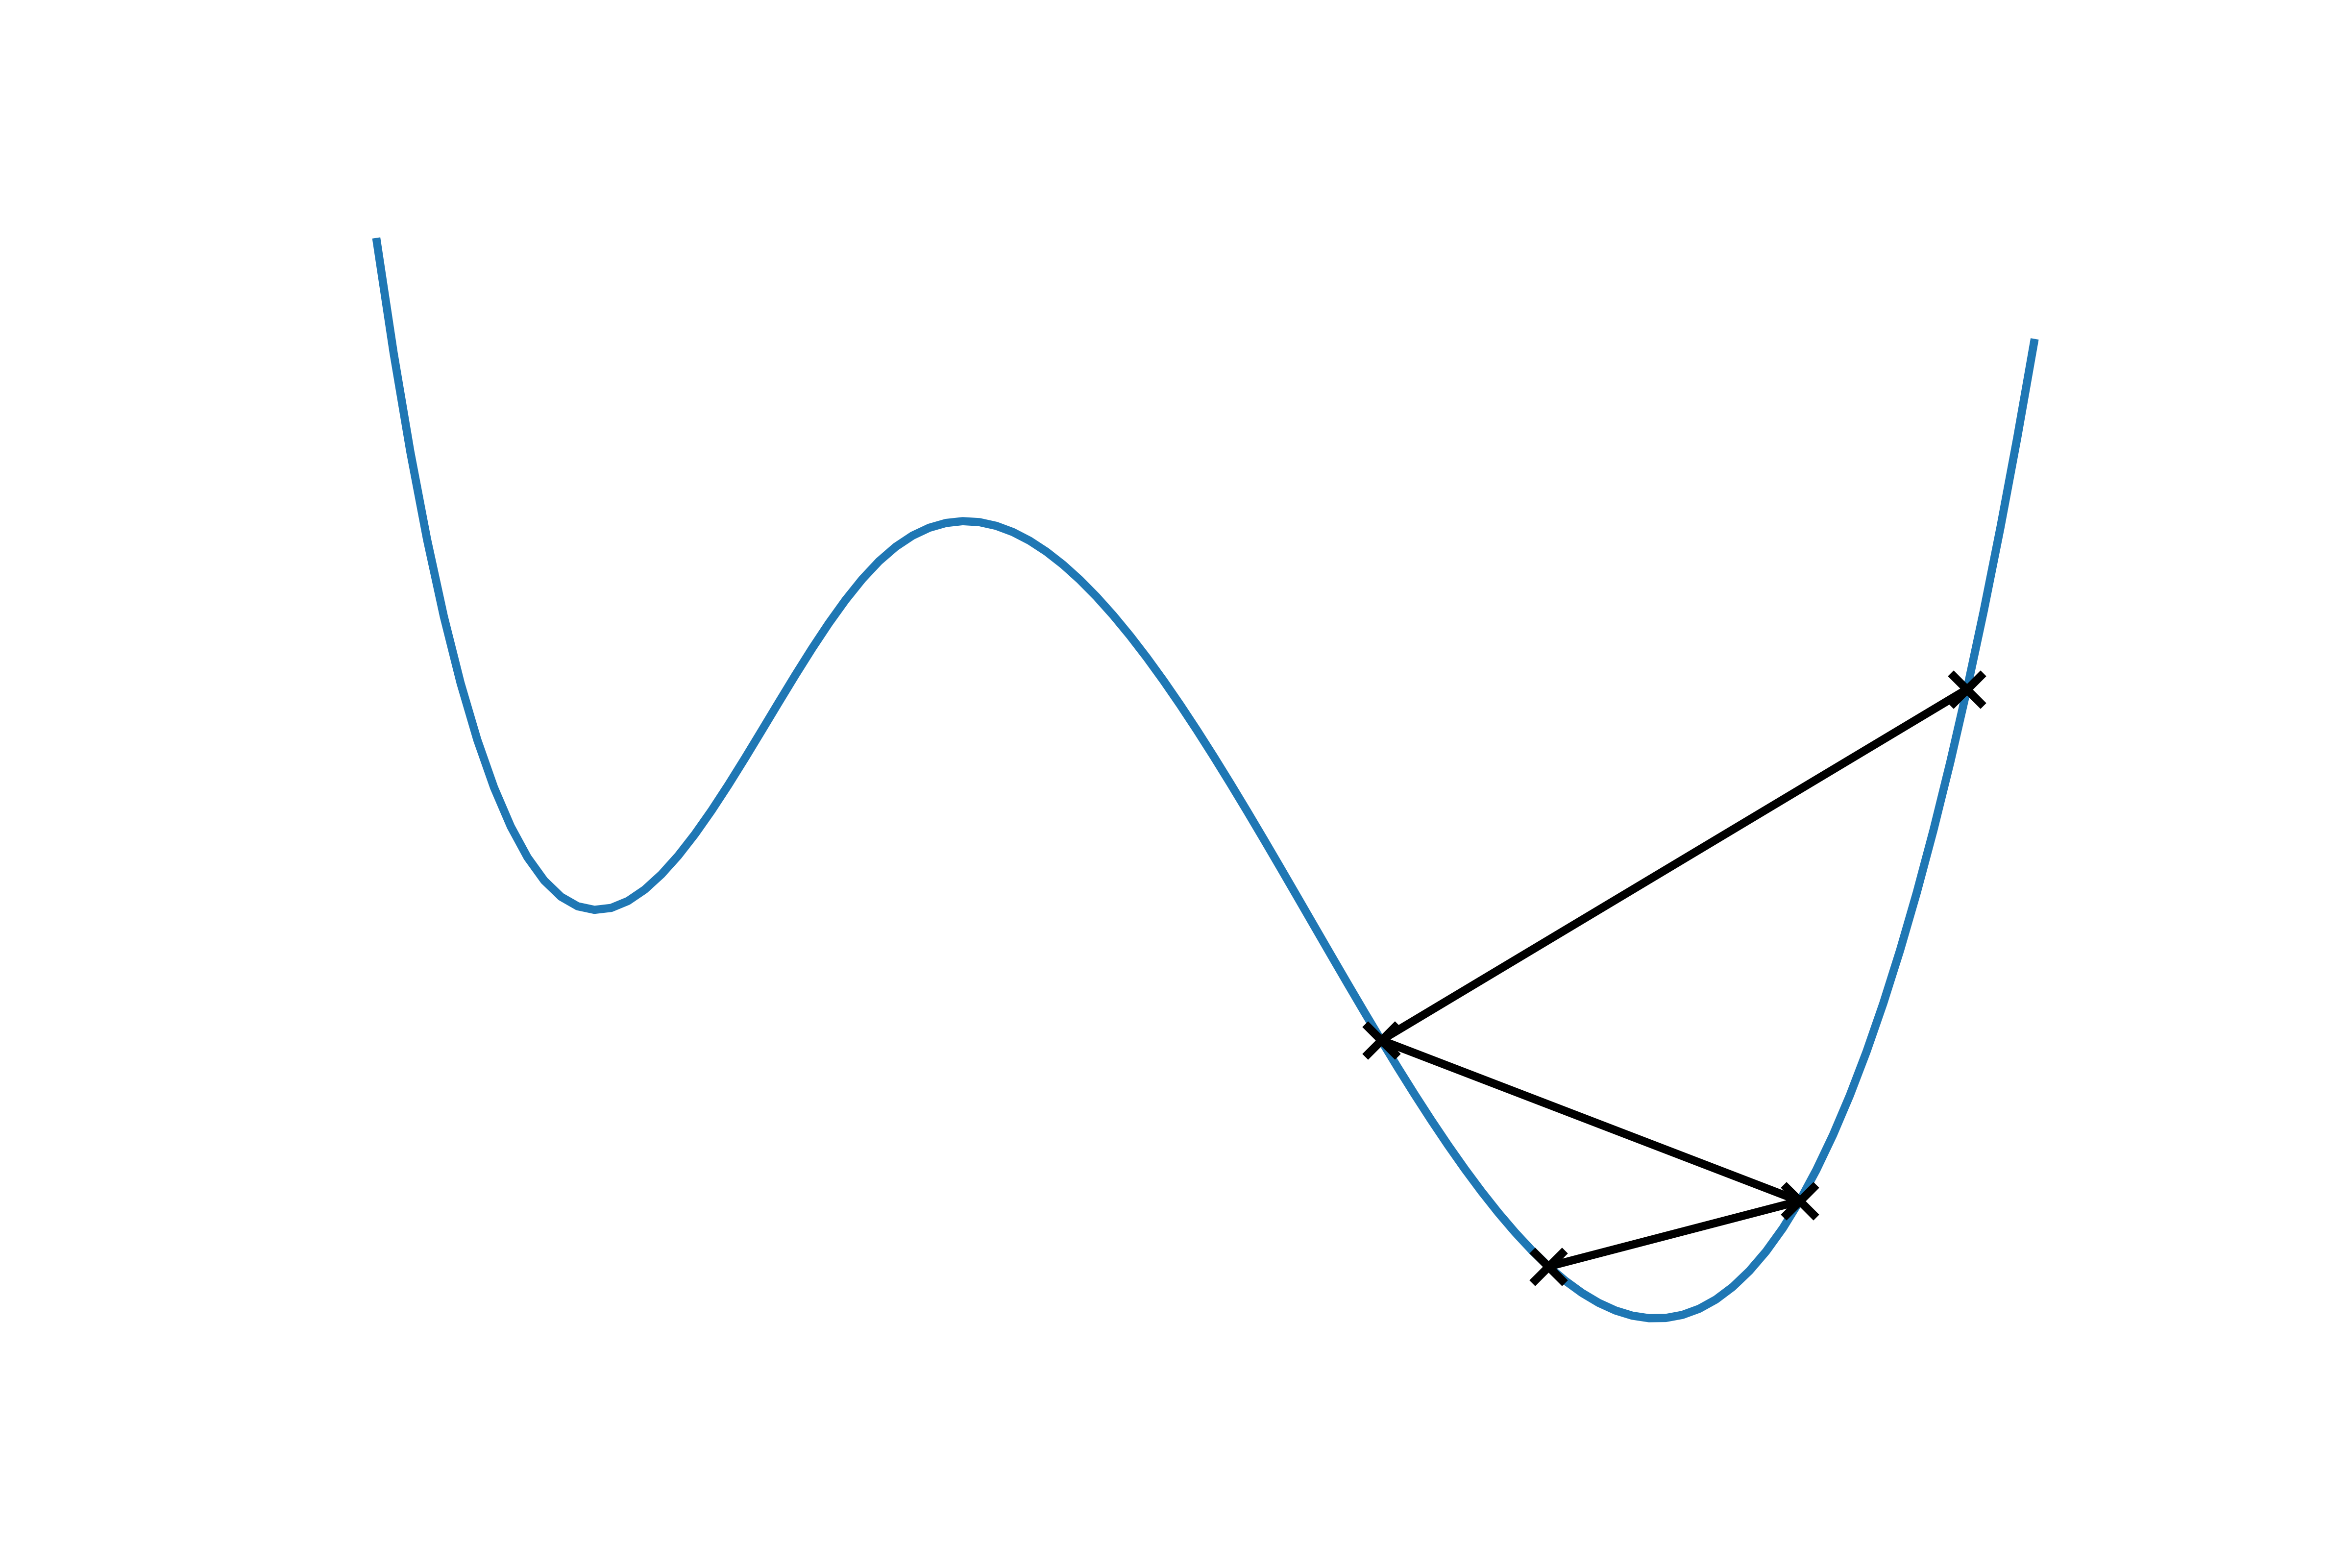
\includegraphics[scale=0.6]{nelder-mead.png}
    \caption{Nelder-mead}
    \label{fig:nelder_mead}
\end{figure}

\begin{figure}
    \includegraphics[scale=0.6]{SLSQP.png}
    \caption{SLSQP}
    \label{fig:slsqp}
\end{figure}

\afterpartskip

\subsection{Results}
\label{subsec:chl_opt_results}

The final parameters for the chl-xTB method are given in table \ref{table:chl_params}.
The best performing set of parameters had an RMSE of excitation energy of, RMSE
of transition dipole magnitude of , and a $R^2$ value of . Repeated optimisation runs
gave parameter and objective function minima to similar values, and the difference in
these values can be attributed to the complex solution space.

It was also found that lower minima of the objective function were found when using
the SLSQP method for optimisation instead of the default Nelder-Mead method. Minima
were found in a smaller number of iterations, reducing the overall CPU time required.
This is in line with benchmarked SLSQP solutions in a non-linear multidimensional space.
It was also investigated whether a reduction in the amount of parameters was possible,
by only training the response parameters and not the Hamiltonian parameters, however 
this did not achieve the same levels of accuracy as using both sets of parameters.

The optimised values do not differ much from the original GFN1-xTB and sTDA-xTB
parameters (given for reference in table \ref{table:chl_params}), with the exception
of the $a_x$ parameter. This parameter is far lower than the sTDA-xTB equivalent,
which has a value of 0.5, noted to be similar to other range-based functional mixing.

\begin{table}
    \centering
    \begin{tabular}{|| l r ||}
    \hline
    Hamiltonian & \\
    $k_\text{s}$ & 1.462 \\
    $k_\text{p}$ & 2.694 \\

    $\text{Mg}_\text{p}$ & 0.902 \\
    $\text{Mg}_\text{s}$ & 1.053 \\
    $\text{N}_\text{p}$ & 1.044 \\
    $\text{N}_\text{s}$ & 1.281 \\

    $\text{Mg}_\text{s}$-$\text{N}_\text{s}$ & 1.468 \\
    $\text{Mg}_\text{s}$-$\text{N}_\text{p}$ & 1.023 \\
    $\text{Mg}_\text{p}$-$\text{N}_\text{s}$ & 1.067 \\
    $\text{Mg}_\text{p}$-$\text{N}_\text{p}$ & 1.402 \\

    \hline\hline
    Response & \\
    $y_K$ & 2.147 \\
    $y_J$ & 4.012 \\
    $a_x$ & 0.067 \\
    $D_{\text{scale}}$ & 0.636\\
    \hline
    \end{tabular}
    \caption{optimized parameters from SLSQP procedure.}
    \label{table:chl_params}
\end{table}

\section{Benchmarking and Cross-validation}
\label{sec:chl_benchmarking}

\subsection{Transition properties}
\label{subsec:transition_properties}

The predicted values for \Qy transition energies are shown against other methods
in figure \ref{fig:training_scatter}. It can be seen that the chl-xTB energies are
well within the range of other DFT functionals, and on a similar level of accuracy
and correlation, which is a huge improvement over the lower level methods.

\begin{figure}
    \includegraphics[scale=0.6]{../../Year_2/chlorophyll_parameterization/training_scatter.png}
    \caption{fig:training scatter}
\end{figure}

\subsection{Potential Energy Surfaces}
\label{subsec:pot_energy_surfaces}

Whilst the stochastic selection of BChla geometries should represent a large section 
of the conformational space in LHII, it is not explicitly given that chl-xTB would
perform equally well all conformations. The errors in transition properties between
PBE0, benchmarked against other DFT methods, and chl-xTB was then calculated for
geometries along multiple normal modes.

The geometries for this test were not taken to be BChla for two reasons. There are
140 of atoms in BChla, giving the number of normal modes is 414, and with
anywhere between 10-20 coordinates along each normal mode this represents a large
number of calculations to do with expensive functionals and basis sets. Additionally,
the normal modes would need to be calculated from an optimised geometry. The phytol
tail in BChla (and chlorophyll in general) make geometry optimisations difficult
due to the large degrees of freedom in rotations along the carbon chain. Therefore
the normal modes and transition properties were calculated for a truncated BChla, 
with a hydrogen atom replacing the phytol tail, instead of a full BChla molecule.

To further reduce the number of calculations needed, only normal modes where strong
coupling to the \Qy transition were taken. It's known that only certain symmetry 
breaking normal modes will couple to the \Qy transition. These can be proxied
by looking at the difference in $N_A$, $N_C$ displacements as the normal mode
is scanned. A plot of these values, as well as the moving average, is shown in figure
\ref{qy_scan}. It is interesting to note that the peaks in the moving average line
closely approximate the peaks in the BChla absorption spectrum.

The modes with highest displacement were then chosen for scans, and the results
are shown in the set of figures.

\begin{figure}
    \includegraphics{../../Year_2/BChla_Qy/Scan_of_Modes.png}
    \label{fig:qy_scan}
\end{figure}

\begin{figure}
    \includegraphics{../../Year_2/BChla_Qy/mode_83.png}
\end{figure}
\begin{figure}
    \includegraphics{../../Year_2/BChla_Qy/mode_85.png}
\end{figure}
\begin{figure}
    \includegraphics{../../Year_2/BChla_Qy/mode_88.png}
\end{figure}
\begin{figure}
    \includegraphics{../../Year_2/BChla_Qy/mode_90.png}
\end{figure}
\begin{figure}
    \includegraphics{../../Year_2/BChla_Qy/mode_91.png}
\end{figure}
\begin{figure}
    \includegraphics{../../Year_2/BChla_Qy/mode_129.png}
\end{figure}
\begin{figure}
    \includegraphics{../../Year_2/BChla_Qy/mode_130.png}
\end{figure}
\begin{figure}
    \includegraphics{../../Year_2/BChla_Qy/mode_132.png}
\end{figure}
\begin{figure}
    \includegraphics{../../Year_2/BChla_Qy/mode_135.png}
\end{figure}
\begin{figure}
    \includegraphics{../../Year_2/BChla_Qy/mode_162.png}
\end{figure}
\begin{figure}
    \includegraphics{../../Year_2/BChla_Qy/mode_169.png}
\end{figure}

\subsection{Absorption Spectra}
\label{subsec:absorption_spectra}

An absorption spectrum for BChla was also calculated with chl-xTB.
In order to account for inhomogeneous broadening, the chlorophyll structures were
taken from an MD simulation of BChla in an explicit ether solvent.

The MD was performed with the \code{OpenMM} toolkit. The chlorophyll structure was
taken from the previously used LHII protein MD, and was packed with diethyl ether.
The forcefield parameters were taken from , using a PME method for the non-bonded
method with a 1 nm cutoff. Equilibriation and production steps were done with a
Langevin integrator, set to 300 K and a timestep of 0.5 femtoseconds. The system
energy was minimised before running a 10ps equilibriation. Frames were then taken
from a 2ns simulation time, with structures taken every picosecond. 

Transition properties for chlorophyll structures from every frame were calculated.
These were calculated using the same methods as included in the reference data.

Absorption spectra, both with and without a single-parameter shift of excitation
energy, can be seen in ref. 

\subsubsection{Particle Mesh Ewald}
\label{subsubsec:PME}
The effect of including embedding effects was also investigated. As the ground
state calculation can include a QM-MM polarisation term in the Fock matrix, non-periodic 
embedding would have been fairly trivial to include. A periodic embedding term could
also be included using an Ewald potential, which uses the relation

\begin{equation}
\frac{1}{r} = 
\end{equation}

